\chapter{Estimación no paramétrica de densidades}

En la estimación de la densidad, como en la Inferencia en general, existen dos posibles vías de estudio.
\begin{itemize}
    \item \textbf{Estimación paramétrica}, en la que se asume determinada distribución de la variable y se emplean datos para la estimación de los correspondientes parámetros.
    \item \textbf{Estimación no paramétrica}, que no asume ninguna distribución, únicamente utiliza la información proporcionada por la muestra.
\end{itemize}
Tanto en la inferencia paramétrica como la no paramétrica poseen numerosos simpatizantes y detractores, pues ambas metodologías de trabajo tienen ventajas e inconvenientes que han sido ampliamente estudiados a lo largo de los años.

La suposicion inicial de que la población de la que proceden los datos sigue un modelo paramétrico puede limitar mucho el ajuste del modelo. En caso deser correcta dicha suposición, el ajuste será muy bueno, pero si el modelo paramétrico es incorrecto, las conclusiones podrían ser totalmente erróneas. Por ello, es deseable considerar técnicas no paramétricas que olviden cualquier hipótesis previa y trabajen únicamente con la información que proporcionan los datos, teniendo siempre presente la aleatoriedad intrínseca a los mismos.

Las principios de la estimación no paramétrica de la densidad datan de finales del siglo XIX, cuando Karl Pearson introdujo el \textbf{histograma}, que no es más que la representación de las frecuencias por clases. El histograma es un estimador discontinuo, que además depende de la elección de un punto inicial y de un parámetro ventana, con gran influencia por parte de ambos en el resultado final.

Para solventar el problema de la dependencia del punto inicial, hay que esperar hasta mediados del siglo XX, cuando se desarrolló el denominado\textbf{ histograma móvil} o \textbf{estimador naive}, que sigue siendo discontinuo y dependiente de la ventana. Posteriormente, Parzen, en 1962, y Rosenblatt (1956), propusieron el estimador tipo núcleo, que sí es continuo y que, por lo tanto, en la mayor parte de las veces, se ajusta mejor a la realidad de los modelos estudiados, aunque también depende en gran medida de la eleccón de un parámetro ventana.

En la literatura estadística ha sido ampliamente estudiado el papel fundamental del parámetro ventana en el estimador tipo núcleo. Dicho parámetro es el que controla el grado de suavización del estimador, y una mala elección del mismo puede derivar en un estimador tanto infra como sobresuavizado. Debido a esto, la segunda mitad del siglo XX fue muy prolífica en cuanto a métodos de seleccioón de ventana, entre los que destacan el propuesto por Silverman (1986), el meétodo de Shealter y Jones (1991) y el de Bowman (1984).

\begin{defi}
    Sea $X_1,\ldots, X_n$ una muestra de datos que proviene de una variable aleatoria $X$ continua con función de densidad desconocida, $f$. El \textbf{estimador de núcleos} de $f$ se define por
    \begin{align*}
        \hat{f}_n(x) = \frac{1}{n} \sum_{i=1}^{n} \frac{1}{h} K\left( \frac{x - X_i}{h}, \right)
    \end{align*}
    donde $K$ es una función, denominada \textbf{función kernel, función núcleo o función peso}, que satisface ciertas condiciones de regularidad, generalmente es una función de densidad simétrica, con media 0 y varianza 1, $h > 0$ es el \textbf{parámetro de suavizado o ancho de banda}.
\end{defi}
El estimador de núcleos se puede ver como una suma de pequeñas montañas o protuberancias
situadas en las observaciones. La funcion núcleo determina la forma de estas protuberancias,
mientras que el paámetro de suavizado determina su anchura.

Cada pequeña montaña o protuberancia está centrada en una observación $X_i$ y tiene una superficie de $1/n$.

Si $h$ es demasiado pequeño, las montañas estarán muy separadas y observaremos muchos picos.

Si $h$ es demasiado grande, observaremos una sola montaña plana.

Un valor intermedio de $h$ debería ser la mejor elección.

Algunas de las funciones núcleo más comunes son
\begin{itemize}
    \item \textbf{Epanechnikov}, $K(t) = \frac{3}{4}(1-t^2)$, $|t| < 1$.
    \item \textbf{Gauss}, $K(t) = \frac{1}{2\pi} e^{-\frac{t^2}{2}}$, $t \in \mathbb{R}$.
    \item \textbf{Triangular}, $K(t) = 1 - |t|$, $|t| < 1$.
    \item \textbf{Rectangular}, $K(t) = \frac{1}{2}$, $|t| < 1$.
    \item \textbf{Biweight}, $K(t) = \frac{15}{16}(1-t^2)^2$, $|t| < 1$.
    \item \textbf{Triweight}, $K(t) = \frac{35}{32}(1-t^2)^3$, $|t| < 1$.
    \item \textbf{Coseno}, $K(t) = \frac{\pi}{4} \cos \left( \frac{\pi t}{2} \right)$, $|t| < 1$.
    \item \textbf{Semicírculo}, $K(t) = \frac{2}{\pi} \sqrt{1 -  t^2}$, $|t| < 1$.
\end{itemize}

\begin{figure}[H]
    \centering
    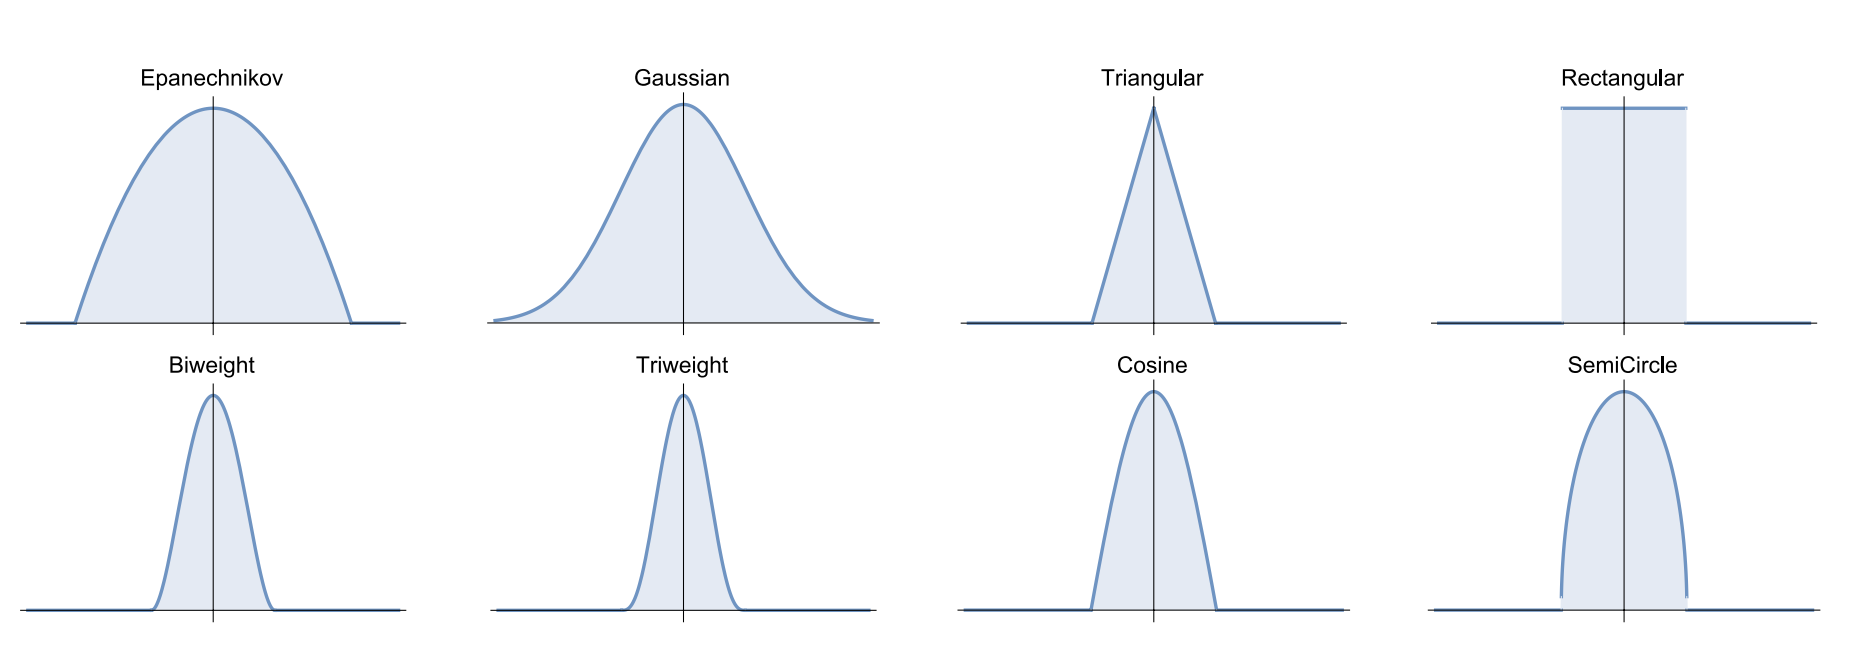
\includegraphics[width=\textwidth]{imagenes6/nucleos.png}
\end{figure}
Apliquemos todo esto a un ejemplo real. Los datos que vamos a analizar fueron analizados en Azzalini y Bowman (1990), (”Applied Smoothing Techniques for Data Analysis”) quienes registraron el tiempo (en minutos) que dura una erupcion´ del geyser Old Faithful que se encuentra en el parque nacional de Yellowstone (Wyoming, USA). Las medidas (27 erupciones en total) fueron tomadas entre el 1 y el 15 de Agosto de 1985.
\begin{figure}[H]
    \centering
    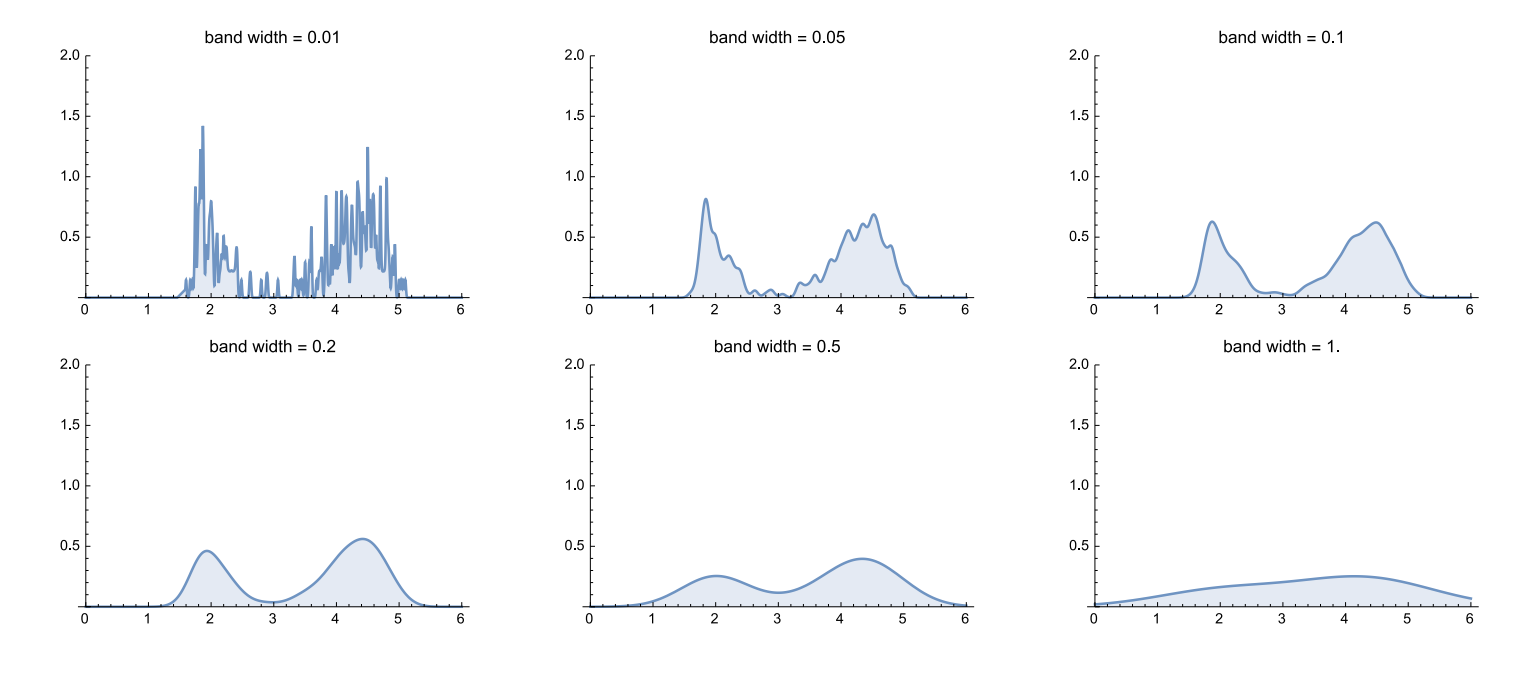
\includegraphics[width=1\textwidth]{imagenes6/nucleo1.png}
    \caption{Ajustando diferentes valores de $h$ con la función núcleo que usa Mathmatica por defecto.}
\end{figure}

\begin{figure}[H]
    \centering
    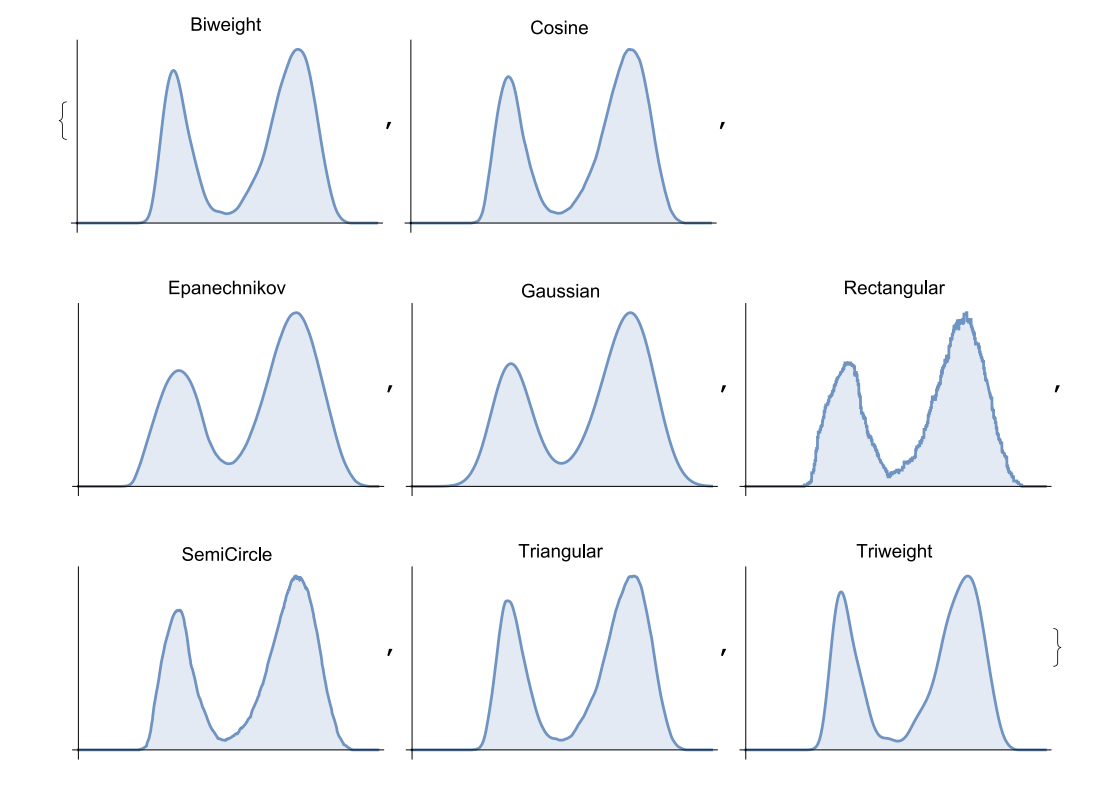
\includegraphics[width=1\textwidth]{imagenes6/nucleo3.png}
    \caption{Funciónes núcleo vistas anteriormente.}
\end{figure}